% !TEX root = *.root.tex

\documentclass[Análisis.root.tex]{subfiles}

\usetikzlibrary{positioning,shapes,fit,arrows}

\begin{document}
    \section{Números reales y Funciones}
    \subsection{Números reales}
        Hasta el momento conocemos distintos conjuntos de números:
        \begin{itemize}
            \item Naturales, \(\mathbb{N} = \{1,2,3,4,...\}\)
            \item Enteros, \(\mathbb{Z} = \{...,-2,-1,0,1,2,...\}\)
            \item Racionales, \(\mathbb{Q} = \{\frac{a}{b} / a \in \mathbb{Z}; b \in \mathbb{Z};b \ne 0\}\)
            \item Reales, \(\mathbb{R}\), como \(\pi\) y \(e\)
        \end{itemize}
        Cada uno de estos conjuntos resulta estar incluido en el anterior:\\[2mm]
        \(\mathbb{N} \subset \mathbb{Z} \subset \mathbb{Q} \subset \mathbb{R}\)
        \begin{center}
            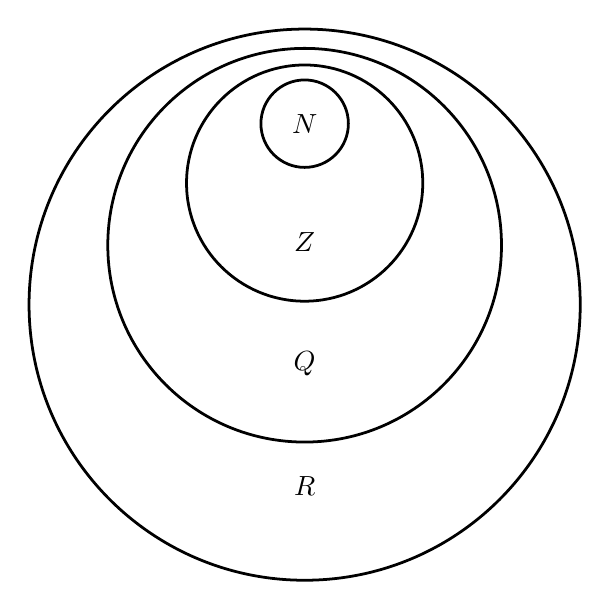
\begin{tikzpicture}[line width=1pt]
                \node (n) {\(\mathbb{N}\)};
                \node [below=of n] (z) {\(\mathbb{Z}\)};
                \node [below=of z] (q) {\(\mathbb{Q}\)};
                \node [below=of q] (r) {\(\mathbb{R}\)};
                \node[shape=circle,draw=black,fit={(n)}] {};
                \node[shape=circle,draw=black,minimum size=3cm,fit={(n) (z)}] {};
                \node[shape=circle,draw=black,minimum size=5cm,fit={(n) (q)}] {};
                \node[shape=circle,draw=black,minimum size=7cm,fit={(n) (r)}] {};
                \draw (n) (z) (q) (r);
            \end{tikzpicture}
        \end{center}
        \subsubsection{Axiomas de cuerpo}
        \subsubsection{Intervalos y otros subconjuntos de la recta real}
        Un intervalo está formado por los números reales que corresponden a los puntos de un segmento o una semirrecta de la recta real. Puede incluir o no a los extremos del segmento o la semirrecta.\\
        Por ejemplo, el conjunto \(A = \{x \in \mathbb{R} / x \geq 1\}\) corresponde a los puntos de la semirrecta hacia la derecha de \(x = 1\), incluyendo a \(x = 1\):
        \begin{center}
            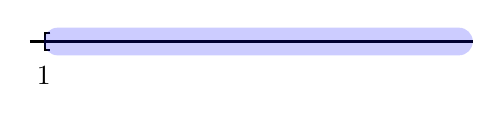
\begin{tikzpicture}[x=5em,y=1em]
                \draw [thick] (-0.1,0) -- (3.1,0);
                \draw [{[-}, thick] (0,0) -- (3.1,0);
                \draw (0, 0) node[below=2mm] {1};
                \fill[opacity = 0.2, blue, rounded corners=.5em] (0,-.5em) -- (3.1, -.5em) -- (3.1, .5em) -- (0,.5em) -- cycle;
            \end{tikzpicture}
        \end{center}
        A este conjunto lo vamos a representar por \(A = [1, + \infty)\).
        El conjunto \(B = \{x \in \mathbb{R} / - 1 < x \leq 2\}\) corresponde a los puntos del segmento comprendido entre \(x = -1\) y \(x = 2\)
        (es decir, los puntos que se hallan a la derecha de \(x = -1\) y simultáneamente a la izquierda de \(x = 2\)), incluyendo a \(x = 2\), pero no a \(x = -1\):
        \begin{center}
            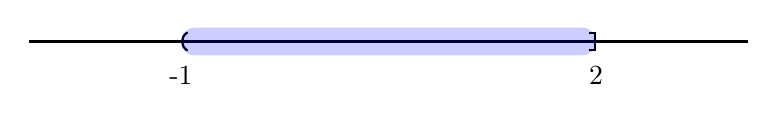
\begin{tikzpicture}[x=5em,y=1em]
                \draw [thick] (-2.1,0) -- (3.1,0);
                \draw [{(-]}, thick] (-1,0) -- (2,0);
                \draw (-1, 0) node[below=2mm] {-1};
                \draw (2, 0) node[below=2mm] {2};
                \fill[opacity = 0.2, blue, rounded corners=.5em] (-1,-.5em) -- (2, -.5em) -- (2, .5em) -- (-1,.5em) -- cycle;
            \end{tikzpicture}
        \end{center}
        En este caso, usamos la notación \(B = (-1; 2]\) para representar a este conjunto.
        \subsubsection{Cotas superiores y supremo}
        Dado un subconjunto \(A\) de números reales, decimos que un número \(K\) es \textit{cota superior} de \(A\) si en la recta todos los elementos de \(A\) están a la izquierda de \(K\). En otras palabra, si todos los elementos de \(A\) son menores o iguales que \(K\): para todo \(a \in A, a \leq K\). Podemos visualizar esta noción en la recta numérica:
        \begin{center}
            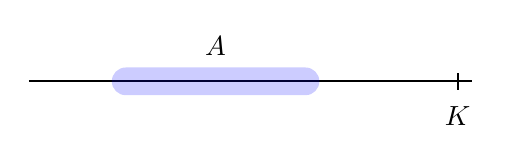
\begin{tikzpicture}[x=5em,y=1em]
                \draw [thick] (-1.1,0) -- (2.1,0);
                \draw [thick] (2,.3) -- (2,-.3);
                \fill[opacity = 0.2, blue, rounded corners=.5em] (-.5,-.5em) -- (1, -.5em) -- (1, .5em) -- (-.5,.5em) -- cycle;
                \draw (2, 0) node[below=2mm] {\(K\)};
                \draw (.25, 0) node[above=2mm] {\(A\)};
            \end{tikzpicture}
        \end{center}
        Si el conjunto \(A\) tiene una cota superior, decimos que \(A\) está \textit{acotado superiormente}, y la menor de todas las cotas superiores se \textit{llama supremo}.\\
        Si \(s\) es el supremo de \(A\) vamos a escribirlo \(s = sup(A)\).\\
        Demos una definición formal de supremo: si \(A\) es un conjunto de números reales, \(s\) es el supremo de \(A\) si verifica las siguientes dos condiciones:
        \begin{itemize}
            \item \(s\) es cota superior de \(A\) y
            \item si \(t\) es otra cota superior de \(A\), entonces \(s \leq t\).
        \end{itemize}
        Otra forma equivalente de definir el supremo es
        \begin{itemize}
            \item \(s\) es cota superior de \(A\) y
            \item si \(r\) es un número real positivo cualquiera, entonces \(s - r\) no es cota superior de \(A\), es decir, siempre exite un \(a \in A\) tal que \(s - r < a \leq s\).
        \end{itemize}
        \subsubsection{Axioma de complejitud}
    \subsection{Funciones}
        Una función \(f: A \rightarrow B\) es una relación entre dos conjuntos, donde cada elemento del conjunto \(A\) señala un sólo elemento del conjunto \(B\).
        \begin{center}
            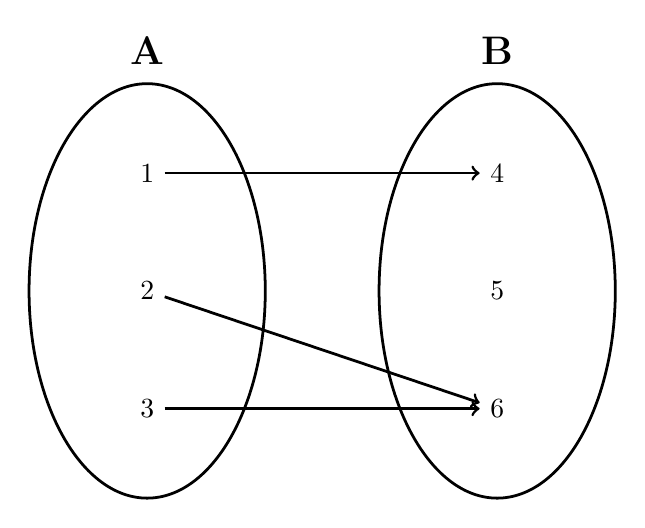
\begin{tikzpicture}[line width=1pt]
                \node (a1) {1};
                \node[below=of a1] (a2) {2};
                \node[below=of a2] (a3) {3};
                \node[right=4cm of a1] (b1) {4};
                \node[below=of b1] (b2) {5};
                \node[below=of b2] (b3) {6};
                \node[shape=ellipse,draw=black,minimum size=3cm,fit={(a1) (a3)}] {};
                \node[shape=ellipse,draw=black,minimum size=3cm,fit={(b1) (b3)}] {};
                \node[above=1cm of a1,font=\Large\bfseries] {A};
                \node[above=1cm of b1,font=\Large\bfseries] {B};
                \draw[->] (a1) -- (b1);
                \draw[->] (a2) -- (b3);
                \draw[->] (a3) -- (b3);
            \end{tikzpicture}
        \end{center}
        Se puede evaluar la función así:
        \begin{center}
            \begin{tabularx}{\textwidth}{XXX}
                \centering{\(f(1) = 4\)} & \centering{\(f(2) = 6\)} & \centering{\(f(3) = 6\)}\\
            \end{tabularx}
        \end{center}
        Como se puede ver, siempre hay un resultado por cada evaluación, no importa si hay dos o más elementos del conjunto \(A\) cuya evaluación tenga el mismo resultado.\\
        En caso contrario, no sería una función, sería una relación no funcional, como el siguiente ejemplo:
        \begin{center}
            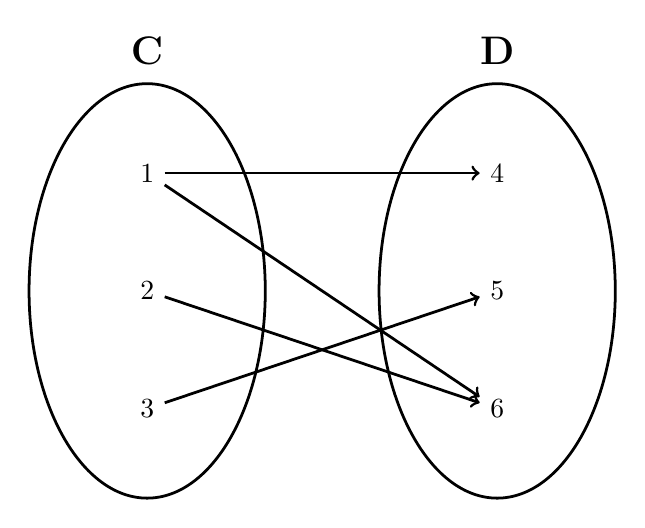
\begin{tikzpicture}[line width=1pt]
                \node (a1) {1};
                \node[below=of a1] (a2) {2};
                \node[below=of a2] (a3) {3};
                \node[right=4cm of a1] (b1) {4};
                \node[below=of b1] (b2) {5};
                \node[below=of b2] (b3) {6};
                \node[shape=ellipse,draw=black,minimum size=3cm,fit={(a1) (a3)}] {};
                \node[shape=ellipse,draw=black,minimum size=3cm,fit={(b1) (b3)}] {};
                \node[above=1cm of a1,font=\Large\bfseries] {C};
                \node[above=1cm of b1,font=\Large\bfseries] {D};
                \draw[->] (a1) -- (b1);
                \draw[->] (a2) -- (b3);
                \draw[->] (a1) -- (b3);
                \draw[->] (a3) -- (b2);
            \end{tikzpicture}
        \end{center}
        Volviendo a las funciones, a todo conjunto de salida se lo denomina el Dominio de una función, en este caso:
        \begin{center}
            \(Dom f = A\)
        \end{center}
        Por su parte, al conjunto de llegada se lo llama el Codominio de una función:
        \begin{center}
            \(Codom f = B\)
        \end{center}
\end{document}